% Created 2023-01-12 Thu 16:16
% Intended LaTeX compiler: lualatex
\documentclass[11pt]{article}
\usepackage{graphicx}
\usepackage{longtable}
\usepackage{wrapfig}
\usepackage{rotating}
\usepackage[normalem]{ulem}
\usepackage{amsmath}
\usepackage{amssymb}
\usepackage{capt-of}
\usepackage{hyperref}
\usepackage{minted}
\usepackage[margin=0.5in]{geometry}
\author{David Lewis}
\date{1/12/2022}
\title{Lec 2: Classroom activity}
\hypersetup{
 pdfauthor={David Lewis},
 pdftitle={Lec 2: Classroom activity},
 pdfkeywords={},
 pdfsubject={},
 pdfcreator={Emacs 28.2 (Org mode 9.6)}, 
 pdflang={English}}
\begin{document}

\maketitle
\section{1}
\label{sec:orgfdc685c}
\begin{enumerate}
\item There are 5 columns (attributes), therefore the dimensionality is 5. There are 8 rows,
therefore the number of points is 8 (in 5 dimensional space).
\item \(\begin{bmatrix} ID2 \\ 23 \\3.5 \\ \text{Masters} \\ \text{Mechanical}\end{bmatrix}\)
\item \begin{itemize}
\item Average GPA: numerical, continuous
\item Level of Education: Categorical, ordinal
\item Major: Categorical, nominal
\end{itemize}
\end{enumerate}
\section{2}
\label{sec:org7431544}
\subsection{a}
\label{sec:orgf4362ae}
1 dimensional scatter plot of points shows the geometric view.
\begin{minted}[fontsize=\scriptsize]{python}
import matplotlib.pyplot as plt
d = [1, 5, 5, 2, 1, 6]
fig, ax = plt.subplots()
ax.scatter(d, [0] * len(d))
ax.yaxis.set_visible(False)
fig.savefig("2a.png")
\end{minted}

\begin{center}
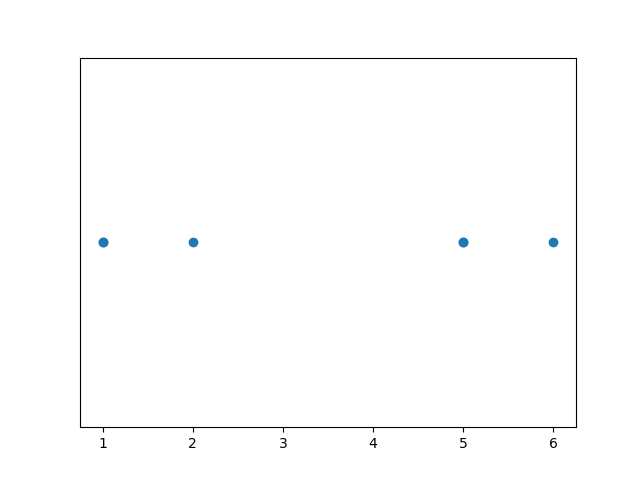
\includegraphics[width=8cm]{2a.png}
\end{center}
\subsection{b}
\label{sec:org1979d5c}
\(\mu = \frac{1+5+5+2+1+6}{6} = \frac{10}{3}\), \(\sigma^2 =
   \frac{(1-\frac{10}{3})^2+(5-\frac{10}{3})^2+(5-\frac{10}{3})^2+(2-\frac{10}{3})^2+(1-\frac{10}{3})^2+(6-\frac{10}{3})^2}{6-1}
   = 1.58 \cdot 10^{31} = 5.067\)
\begin{minted}[fontsize=\scriptsize]{python}
u = 10/3
return (((1-u)**2) + ((5-u)**2) + ((5-u)**2) + ((2-u)**2) + ((1-u)**2) + ((6-u)**2))/(6-1)
\end{minted}


\subsection{c}
\label{sec:org8ef546e}
Three points with lower x and higher y are clustered together as well as three
points with higher x and higher y are clustered together.
\begin{minted}[fontsize=\scriptsize]{python}
import matplotlib.pyplot as plt
d = {"score1":[1, 5, 5, 2, 1, 6], "score2":[4, 1, 0, 4, 5, 1]}
fig, ax = plt.subplots()
ax.scatter(d["score1"], d["score2"])
fig.savefig("2c.png")
\end{minted}

\begin{center}
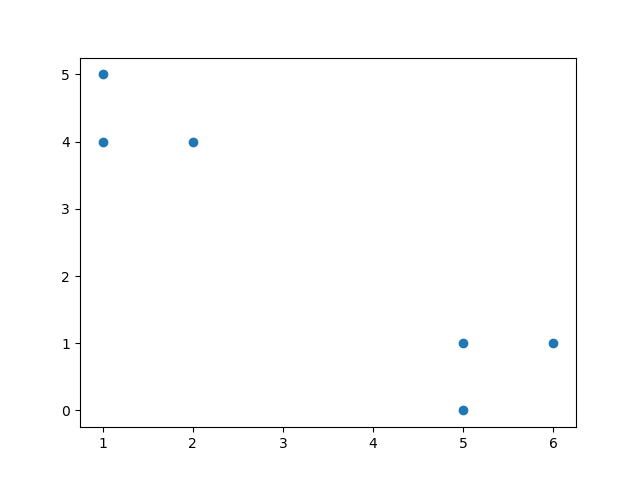
\includegraphics[width=8cm]{2c.png}
\end{center}
\subsection{d}
\label{sec:org18b72e8}
The formula for \(\cos \theta\) is \(\frac{a \cdot b}{||a||||b||}\) where a and b are
vectors with the same dimesionality. Implementing this in python using the given points:
\begin{minted}[fontsize=\scriptsize]{python}
d = tuple(zip([1, 5, 5, 2, 1, 6],[4, 1, 0, 4, 5, 1]))
import math

def dot(a, b):
    return a[0]*b[0] + a[1]*b[1]

a = {}
def length(a):
    return math.sqrt((a[0]**2) + (a[1]**2))

def cos(x, y):
    return dot(d[x-1], d[y-1])/(length(d[x-1]) * length(d[y-1]))
a["1,5"] = cos(1, 5)
a["1,6"] = cos(1, 6)
a["2,6"] = cos(2, 6)
a["3,5"] = cos(3, 5)
return list(a.items())

\end{minted}

\begin{center}
\begin{tabular}{lr}
1,5 & 0.9988681377244377\\
1,6 & 0.39872611141445\\
2,6 & 0.9994801143396996\\
3,5 & 0.19611613513818404\\
\end{tabular}
\end{center}
\subsection{e}
\label{sec:org37fa21d}
\begin{minted}[fontsize=\scriptsize]{python}
d = tuple(zip([1, 5, 5, 2, 1, 6],[4, 1, 0, 4, 5, 1]))
import math
def dist(p1, p2):
   p1 = d[p1-1]
   p2 = d[p2-1]
   return math.sqrt(((p1[1]-p2[1])**2) + ((p1[0] - p2[0])**2))

a = {}
a["1,4"] = dist(1, 5)
a["1,5"] = dist(1, 6)
a["2,6"] = dist(2, 6)
a["4,6"] = dist(4, 6)
return list(a.items())

\end{minted}
\subsection{f}
\label{sec:org6bbd8a3}
The values along the diagonal are all equal for both matrices.
\section{3}
\label{sec:org3514a77}
\begin{enumerate}
\item 4.6 ( the third element of the mean vector )
\item 3.58 ( along the diagonal on the second column )
\item -3.67 ( 1st row, second column or vice versa )
\item The negative covariance implies that the two variables (score 1 and 2) are
inversly related, they move away from each other. The magnitude is larger than the covariance between score 1
and 3 and 2 and 3, meaning that the relationship between 1 and 2 is more
significant than the other relationships (they affect each other more). This
means that the linear relationship is stronger.
\item correlation forumula is \(\frac{\sigma_{xy}}{\sqrt{\sigma^2_x \sigma^2_y}} \rightarrow
   \frac{-3.67}{\sqrt{4.22 \cdot 3.58}} = -0.944\)
\item The negative sign indicates an inverse relationship. The magnitude is close
to one, indicating that the linear relationship between score 1 and 2 is strong.
\end{enumerate}
\section{Bonus}
\label{sec:org2fc83fd}
Correlation is the normalized/standardized covariance. They both show the type of linear
relationship with their sign (positive or negative) and they share the meaning
of the sign. The significant difference between correlation and covariance is
that the correlation is equal to the cosine of the angle between the two centered
attribute vectors.
\end{document}
